\chapter{ANÁLISE DE RUPTURA DE BARRAGENS}
%Título Capítulo 5 

Como pôde ser observado nos capítulos anteriores, a ruptura de barragens possui, além de aplicações práticas, importância científica. Neste contexto, este capítulo faz uma análise sobre esse fenômeno iniciando com uma visão geral sobre o assunto, Seção \ref{visao}. Prossegue destacando o trabalho de \citeonline{Crespo}, Seção \ref{arte}. Destaca a construção de um modelo unidimensional baseado nas equações de Euler, Seção \ref{Modelo1D} e obtém uma solução analítica unidimensional para as equações de Águas Rasas, Seção \ref{ModeloAR}. Depois, Seção \ref{py}, disserta sobre o código numérico PySPH, como foi realizado o tratamento de uma barragem hipotética e os resultados obtidos. Por fim, descreve como o assunto foi abordado nesta dissertação, Seção \ref{proposta} e a forma como foi desenvolvida a malha computacional, Seção \ref{malha}. 
    

\section{VISÃO GERAL DE UMA BARRAGEM HIPOTÉTICA} \label{visao}

Considerando seu valor científico, a modelagem da ruptura de uma barragem hipotética tem sido útil como forma de validação de muitos algoritmos numéricos, assim como foi feito no trabalho de \citeonline{CrespoBondary}.

Uma barragem pode ser representada como um tanque que, em seu interior, separa dois níveis de água. O nível com maior volume representa o reservatório (montante) e o de menor nível representa o leito do rio (jusante). Como exemplo desta representatividade pode-se destacar o trabalho realizado por \citeonline{Stansby} que construíram, em laboratório, um reservatório com diferentes níveis de água e capturaram, por meio de uma câmera de vídeo, os estágios iniciais da frente de onda formada pelo colapso daquela estrutura, Figura \ref{fig:captura}.

\begin{figure}[H]
\centering
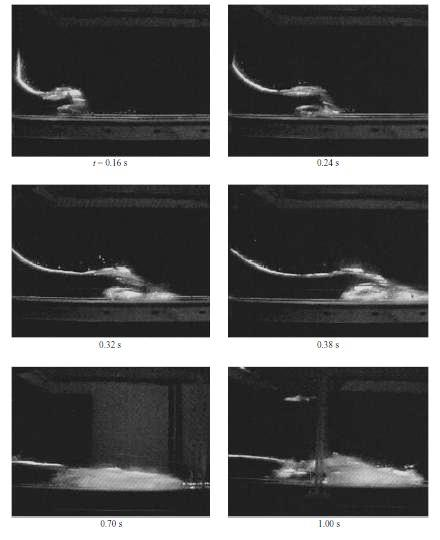
\includegraphics[scale=1]{figuras/captura.jpg}
\caption{\textsc{Captura dos estágios iniciais da simulação da ruptura de uma barragem em laboratório}}
\vspace{-0.1cm}
\legend{FONTE: \citeonline{Stansby}}
\label{fig:captura}
\end{figure}

Experimentos como esse são denominados de modelagem em "leitos úmidos", pois a jusante da barragem há uma fina camada de água, representado o leito do rio, no qual se deposita a água do reservatório no momento da falha da estrutura que as separa. Ao contrário disso, quando a jusante da barragem o leito não contém nenhuma lâmina d'água, denomina-se "leito seco". \citeonline{Korobkin} estudaram os estágios iniciais desse fenômeno e o resolveram analiticamente para pequenos intervalos de tempo, com o intuito de verificar o comportamento da linha de frente da coluna d'água. 

Em ambos experimentos os autores definiram a simulação da ruptura de barragens como uma massa líquida que, inicialmente em repouso, entra em movimento sob os efeitos da gravidade. Como os campos de pressões são diferentes, à montante um campo de pressão hidrostática, equação (\ref{eqhidro}), e à jusante a pressão atmosférica, no caso de um leito seco, ocorre um ajustamento entre eles, resultando em movimentos instáveis, conforme destacam \citeonline{Stansby}.

Quando a simulação é feita sob a hipótese de um leito úmido, a pressão a jusante também é hidrostática, mas as variações são menores devido à profundidade do leito. Neste caso, o comportamento da coluna d'água que se deposita sobre o leito do rio forma o que os pesquisadores denominam de frente de onda ou de inundação, largamente estudada pelos interessados em verificar o comportamento de ondas que atingem regiões costeiras ou por aqueles que desejam obter respostas sobre erosões que esses fenômenos pode causar em estruturas localizadas em regiões de risco. A Figura \ref{fig:stans6} mostra a formação dessas ondas para diferentes intervalos de tempo, destacando o contraste do fenômeno para diferentes profundidades do leito e, também, quando o leito é considerado seco.    

\begin{figure}[H]
\centering
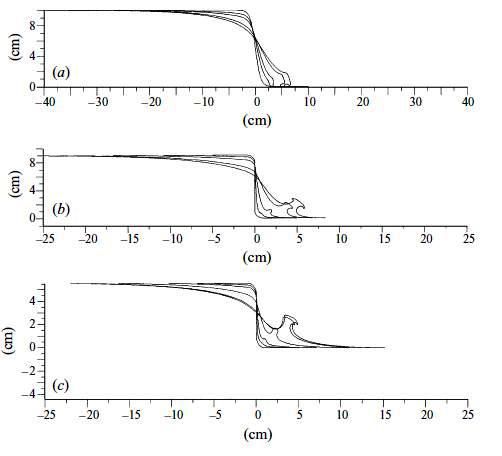
\includegraphics[scale=1]{figuras/stans6.jpg}
\caption{\textsc{Perfil da superfície de elevação para um escoamento potencial não linear em diferentes intervalos de tempo e profundidades}}
\vspace{-0.1cm}
\legend{FONTE: \citeonline{Stansby}}
\label{fig:stans6}
\end{figure}

A forma de tratar as condições iniciais e de contorno podem variar de acordo com a configuração adotada, seja euleriana ou lagrangeana, assim como a inserção de efeitos viscosos ou variações nas densidades. Para o caso de uma simulação usando SPH, por exemplo, existe a necessidade da adoção de uma viscosidade artificial que previna as instabilidades no movimento dos fluidos \cite{Monaghan1992}. Isso faz com que o tratamento das equações governantes do sistema varie em cada configuração e, também, dentro de uma mesma configuração, mas conduz a resultados quase sempre satisfatórios.  

%-------------------------------------------------------------------------------------------------------------------------------------------------------
\section{O ESTADO DA ARTE} \label{arte}

Para simular a ruptura de uma barragem hipotética utilizando as equações de Euler, discretizadas pelo MDFE, foi utilizado, como referência, o trabalho desenvolvido por \citeonline{Crespo}, onde autores estudaram a formulação clássica do SPH para problemas de escoamentos em superfícies livres investigando as variações de filtros de densidade, núcleos, as correções dos gradientes, viscosidades e as condições de fronteiras, como as partículas fantasmas e as partículas dinâmicas. 

Para testar seus resultados consideraram a barragem hipotética adotada por \citeonline{Koshizuka}, sendo que essa é montada em um tanque bidimensional com $4 \ m$ de comprimento, $3 \ m $ de altura e possui uma coluna d'água com $1 \ m$ de comprimento e $2 \ m$ de altura que simula o reservatório. A Figura \ref{fig:tanque} mostra a configuração inicial do sistema que, conforme pode ser observado, foi considerado como uma simulação para leito seco.

\begin{figure}[H]
\centering
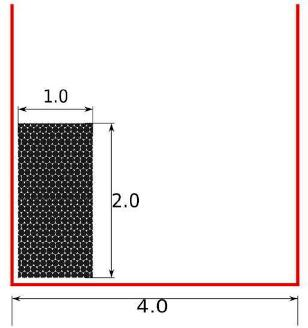
\includegraphics[scale=1]{figuras/tanque.jpg}
\caption{\textsc{Configuração inicial da coluna d'água e do tanque}}
\vspace{-0.1cm}
\legend{FONTE: \citeonline{Crespo}}
\label{fig:tanque}
\end{figure}

\citeonline{Crespo} resolveram o sistema utilizando um algoritmo preditor-corretor descrito no trabalho de \citeonline{Monaghan1989}. Consideraram núcleos formados pelas funções Spline cúbicas, condições de fronteira dinâmica, viscosidade artificial, $\alpha = 0,5$, e fator de correção XSPH, $\epsilon = 0,5$, que calcula uma média entre as velocidades das partículas vizinhas permitindo um escoamento mais suave e evitando a desordem entre as partículas \cite{Paiva2009}.

Como primeira simulação, consideraram um caso padrão adotando a discretização nos eixos coordenados $x$ e $z$ como $dx=dz=0,012 \ m$, tamanho da suavização do núcleo igual a $h=0,0156 \ m$, formando $29.723$ partículas, sem filtro de densidade ou fator de correção. A Figura \ref{fig:colapso} mostra a evolução das velocidades da coluna d'água para diferentes intervalos de tempo, destacando as velocidades no fundo, próximas da barragem, que são máximas. Destacam também, a formação do \textit{sloshing} quando ocorre a colisão com o muro direito.

\begin{figure}[H]
\begin{center}
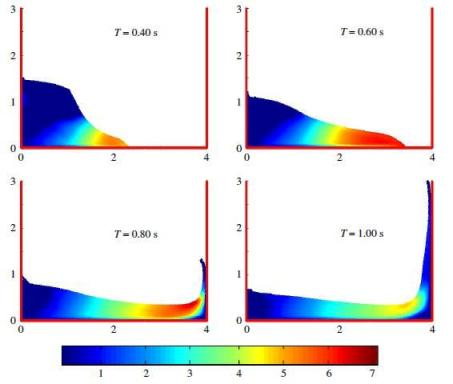
\includegraphics[scale=1]{figuras/colapso.jpg}
\end{center}
\caption{\textsc{Simulação em SPH das velocidades das partículas no colapso de uma coluna d'água}}
\vspace{-0.1cm}
\legend{FONTE: \citeonline{Crespo}}
%\fonte{\citeonline{Crespo}}
\label{fig:colapso}
\end{figure}   

Mais alguma conclusões são obtidas com este experimento, principalmente no que se refere as oscilações de pressão que, segundo os autores, podem ser suavizadas com o uso de filtros sobre a densidade. Assim, a Figura \ref{fig:sfiltro} destaca as variações da densidade em três intervalos de tempo, enfatizando o momento em que a massa líquida entra em contato com o muro, onde ocorre o maior aumento na densidade, $T=0,70s$, e, consequentemente, uma rápida queda de pressão que pode desestruturar os cálculos em todos os campos considerados. No entanto, com a utilização de filtros de densidade, conseguiram melhorar estas diferenças, sem muita interferência na forma física do problema, como pode ser notado nas Figuras \ref{fig:cfiltroS} e \ref{fig:cfiltroM} que mostram a evolução da densidade com dois filtros diferentes para o mesmo intervalo de tempo.

\begin{figure}[H]
\centering
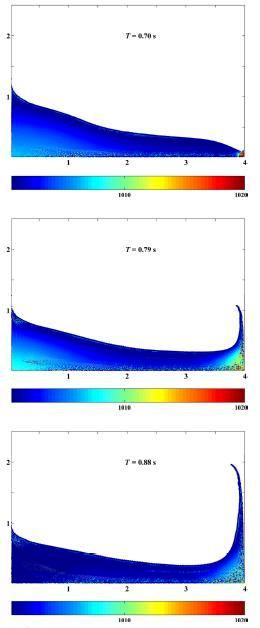
\includegraphics[scale=1]{figuras/sfiltro.jpg}
\caption{\textsc{Evolução da densidade sem a adoção de filtro de correção ao colidir com o muro}}
\vspace{-0.1cm}
\legend{FONTE: \citeonline{Crespo}}
\label{fig:sfiltro}
\end{figure}

\begin{figure}[H]
\centering
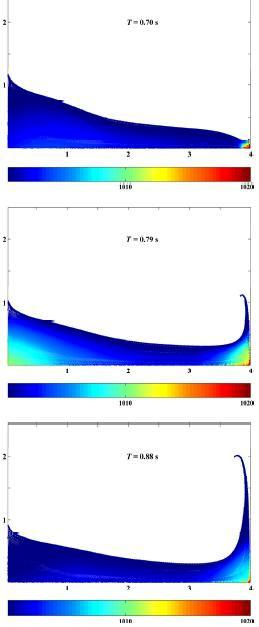
\includegraphics[scale=1]{figuras/cfiltroS.jpg}
\caption{\textsc{Evolução da densidade com a adoção de filtro de correção de Shepard ao colidir com o muro}}
\vspace{-0.1cm}
\legend{FONTE: \citeonline{Crespo}}
\label{fig:cfiltroS}
\end{figure}

\begin{figure}[H]
\centering
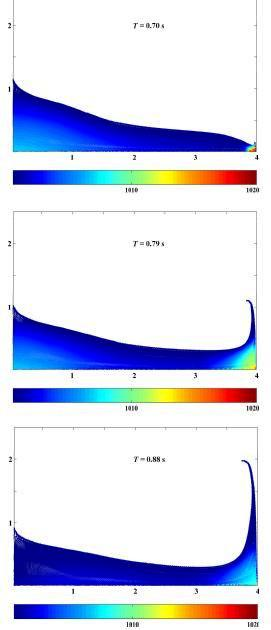
\includegraphics[scale=1]{figuras/cfiltroM.jpg}
\caption{\textsc{Evolução da densidade com a adoção de filtro de correção MLS ao colidir com o muro}}
\vspace{-0.1cm}
\legend{FONTE: \citeonline{Crespo}}
\label{fig:cfiltroM}
\end{figure}

Nesse trabalho, os autores ainda consideraram a simulação da ruptura de uma barragem para o caso de leito úmido, onde observaram o comportamento da frente de onda e, também, adotaram obstáculos a jusante da barragem, mas estes experimentos fogem do escopo desta dissertação.        
%---------------------------------------------------------------------------------------------
\section{MODELO UNIDIMENSIONAL} \label{Modelo1D}

Para a construção de um modelo unidimensional das equações de Euler conservativa, equações (\ref{massasis}) a (\ref{energiasis}),  foi utilizada uma adaptação do canal finito, Figura \ref{fig:tanque}, considerado em \citeonline{Crespo}.  

\begin{figure}[H]
	\centering
	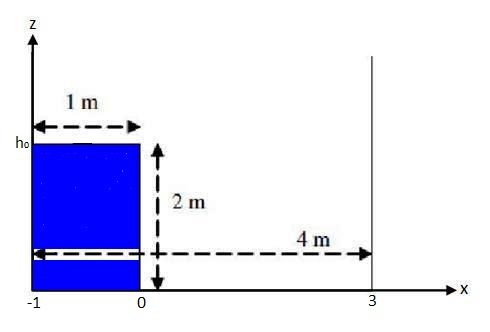
\includegraphics[scale=1]{figuras/tanque2.jpg}
	%\ includegraphics[width=.4\textwidth]{tanque2.jpg}
	\caption{\textsc{Canal finito simulando uma barragem hipotética}}
	\vspace{-0.1cm}
	\legend{FONTE: Adaptado de \citeonline{Crespo}}
	\label{tanque2}
\end{figure}

A modificação realizada, Figura \ref{tanque2}, define que a barragem está representada na origem do sistema cartesiano, $x=0$, separando dois níveis de leitos. À montante da barragem, $x<0$ , encontra-se o reservatório, com altura da coluna d'água igual a $h(x,0)=2 \ m$. À jusante, $x>0$, tem-se o leito seco, com altura da coluna d'água igual a $h(x,0)=0 \ m$. Essas diferenças nos leitos, conforme comentado na Seção \ref{visao}, formam níveis de transição nas propriedades físicas do escoamento e podem ser tratadas, matematicamente, como descontinuidades das quantidades físicas. Se essas descontinuidades não forem adequadamente modeladas irão conduzir a soluções espúrias.

Como passo inicial na formulação unidimensional, considera-se o escoamento incompressível, com a densidade $\rho = \text{constante}$ e o movimento da massa líquida ocorrendo somente na direção do eixo coordenado $x$. Dessa forma, as equações de conservação da massa e do momento nas equações de Euler, equações (\ref{massasis}) e (\ref{momentox}), serão escritas como
\begin{equation}\label{UIncomp}
u_x=0
\end{equation}
e 
\begin{equation} \label{momenIncomp}
\rho u_t + (\rho u^2 + P)_x = 0.
\end{equation}

Integrando a equação (\ref{UIncomp}) em função de $x$, resulta
\begin{equation} \label{Uf}
u(x,t)= f_1 (t),
\end{equation}
que independe de $x$.

Derivando a equação (\ref{Uf}) em função do tempo $t$ e substituindo o resultado encontrado na equação (\ref{momenIncomp}), obtêm-se
\begin{equation} \label{ContModif}
\rho f^{'}_{1}(t)+ P_x =0.
\end{equation}

Utilizando a hipótese de pressão hidrostática, equação (\ref{varpres}), e que a mesma é uma média da profundidade do canal, pode-se considerar que
\begin{equation}\label{PressaoMedia}
P = \rho g \frac{h(x,t)}{2}.
\end{equation} 

Substituindo a equação (\ref{PressaoMedia}) na equação (\ref{ContModif}), encontra-se
\begin{equation}\label{Derh}
\rho f^{'}_{1}(t) + \frac{\rho g}{2} h_x=0.
\end{equation}

Fazendo as devidas simplificações na equação (\ref{Derh}) e integrando o resultado em função de $x$, determina-se o perfil da superfície livre dado por
\begin{equation} \label{EQFINAL}
h(x,t) = \frac{-2f^{'}_{1}(t)x}{g} + f_2(t).
\end{equation}

Nos contornos do canal, Figura \ref{tanque2}, tem-se que $u(l,t)=0$ e $u(L,t) = 0$. Como $u(x,t)=f_1(t)$ independe de $x$, a equação (\ref{EQFINAL}) não terá solução. Isso mostra que a forma como foi construído o modelo unidimensional, usando as equações de Euler sob a hipótese de escoamento incompressível em canais finitos, não soluciona o problema da ruptura de barragens em questão.

%---------------------------------------------------------------------------------------------
\section{MODELO DE ÁGUAS RASAS} \label{ModeloAR}

O tratamento adotado para o modelo unidimensional, apresentado Seção \ref{Modelo1D}, mostrou não ser possível obter uma solução para o problema da ruptura de barragens utilizando a hipótese de escoamento incompressível em canais finitos. No entanto, em 1892, Ritter obteve uma solução para o problema considerando a hipótese de canais retangulares e infinitos \cite{Sakkas}. Essa solução foi determinada baseando-se no Método das Características \cite{Zenchuk} e \cite{Henderson}. Para tanto, seja
\begin{equation} \label{velonda}
c(x,t)= \sqrt{gh}
\end{equation}
a velocidade de propagação de uma onda, sendo $h \geq 0$ a profundidade total da superfície livre e $g$ a aceleração da gravidade. 

Multiplicando a equação de Águas Rasas (\ref{ARR2}) por $g$ e considerando, na equação (\ref{velonda}), que $c^2 = gh$, tem-se
\begin{equation} \label{ARR3}
(c^2)_t + (uc^2)_x = 0.
\end{equation} 

Derivando a  equação (\ref{ARR3}) e realizando as devidas simplificações, encontra-se
\begin{equation} \label{ARFim}
(2c)_t + u(2c)_x + cu_x = 0.
\end{equation}

Novamente, na  equação (\ref{velonda}), considerando que $h = {c^2}/{g}$ e substituindo na equação de Águas Rasas (\ref{AR2}), defini-se que
\begin{equation}\label{AR3}
u_t +uu_x + g \left( \frac{c^2}{g} \right)_x= 0.
\end{equation}

Sabendo que a derivada de $h = {c^2}/{g}$, em função de $x$, resulta em $h_x = 2cc_x /g$, a substituição desse resultado irá transformar a equação (\ref{AR3}) em
\begin{equation} \label{ARFim2}
u_t + uu_x + 2cc_x = 0.
\end{equation}

As equações (\ref{ARFim}) e (\ref{ARFim2}) formam o modelo de Águas Rasas unidimensional baseado na velocidade do escoamento $u$ e na velocidade de propagação da onda $c$. Somando e subtraindo essas equações resultará em um par de EDPs
\begin{equation}\label{SomAR}
\left[ \frac{ \partial}{ \partial t} + (u \pm c) \frac{ \partial}{ \partial x} \right](u \pm 2c) =0.
\end{equation}

Se, na equação (\ref{SomAR}) for considerado que
\begin{equation*}
\frac{d}{dt}(u \pm 2c) = 0,
\end{equation*}
então
\begin{equation*}
\frac{dx}{dt} = (u \pm c).
\end{equation*}

Desse resultado pode-se interpretar, por meio do Método das Características, que as inclinações das linhas características $ C^+ $ são definidas como
\begin{equation*}
\left. \frac{dx}{dt} \right|_{C^+} = (u + c)
\end{equation*}
e que, ao longo dessas linhas, $u + 2c = \text{constante}$.

De forma análoga, pode-se interpretar que as inclinações das linhas características $C^-$ são determinadas por
\begin{equation*}
\left. \frac{dx}{dt} \right|_{C^-} = (u - c)
\end{equation*}
e que, ao longo dessas linhas, $u - 2c = \text{constante}$.

As funções $u+2c$ e $u-2c$ são chamadas de invariantes de Riemann e se propagam, quer à montante $(-c)$ ou à jusante $(+c)$, em relação à velocidade do fluxo $u$.   

Uma classe especial de solução, chamada de onda simples, surge quando uma das invariantes de Riemann é sempre constante no domínio de interesse. Neste caso, se for considerada a propagação da uma onda, movendo-se para a direita, em águas estacionárias e com profundidade constante, $z=h$, então todas as linhas características $C^-$ surgirão da região não perturbada, conforme pode ser observado na Figura \ref{219B}. Além disso, como $u_0=0$ e $c_0 = \sqrt{gh_0}$, então a invariante de Riemann nessa região será
\begin{equation} \label{Equau}
u-2c=u_0 - 2c=-2c_0.
\end{equation}
Assim, $u-2c$ será sempre constante e, como $u+2c$ é constante nas linhas características $C^+$, irá implicar em $u$ e $c$ também constantes nas linhas $C^+$. 

\begin{figure}[H]
	\centering
	\includegraphics[scale=1]{figuras/219B.jpg}
	%\fbox{\includegraphics[width=.4\textwidth]{219B.jpg}}
	\caption{\textsc{As linhas características $C^+$ e $C^-$ para uma onda se propagando para direita numa região estacionária e de profundida constante}}
	\vspace{-0.1cm}
	\legend{FONTE: \citeonline{Johnson}}
	\label{219B}
\end{figure}

A forma de interpretar o caso da onda simples serve para compreender a estruturação da solução no caso da ruptura de barragens. Se for considerado que, para o tempo $t=0$, ocorre o colapso da estrutura localizada na origem do sistema $x=0$ e, nesse instante, 
\begin{equation*}
u= u_0 =0
\end{equation*}
e
\begin{equation*}
h(x, 0) = \left\{
	\begin{array}{rcl}
	h_0 \ ; \ x<0 &  & \\
	& & \\
	0 \ ; \ x>0 &  &, 
	\end{array} \right.
\end{equation*}
sendo $h_0>0$  constante, todas as características virão da região não perturbada $x<0$ e serão constantes, ou seja, 
\begin{equation*}
u+2c=2 \sqrt{gh_0}.
\end{equation*}

No momento em que se inicia o movimento da massa líquida irão surgir infinitas linhas características da origem $x=0$, todas com inclinações diferentes, pois cada $h$, $0 \leq h \leq h_0$, determina uma linha característica. Então, para tratar o fenômeno, há a necessidade de uma forma degenerada da solução característica.

Das linhas características $C^-$ tem-se que suas inclinações são
\begin{equation}\label{IncliC}
\frac{dx}{dt} = u-c,
\end{equation}
onde $u-2c$ é constante. Mas, $u+2c$ é constante e, assim, pode-se concluir que $u$, $c$, $u-c$ são constates e $C^-$ são linhas retas. Com isso, integrando a equação (\ref{IncliC}), em função de $t$, encontra-se
\begin{equation}\label{IntC}
x= (u-c)t,
\end{equation}
o que indica que todas estas linhas características $C^-$ irão passar pela origem do sistema $(0,0)$. Este comportamento das linhas características é chamado de leque de expansão, conforme mostra a Figura \ref{220B}.

\begin{figure}[H]
	\centering
	\includegraphics[scale=1]{figuras/220B.jpg}	%\fbox{\includegraphics[width=.4\textwidth]{220B.jpg}}
	\caption{\textsc{As linha características $C^+$ e $C^-$ para o problema da ruptura de barragens}}
	\vspace{-0.1cm}
	\legend{FONTE: \citeonline{Johnson}}
	\label{220B}
\end{figure}

Da condição inicial em que $u(0)=0$, tem-se
\begin{equation} \label{CDini}
u+2c=2 \sqrt{gh_0}= 2c_0,
\end{equation}
ou seja,
\begin{equation} \label{condi1}
u= 2c_0 -2c.
\end{equation}

Da hipótese de todas as linhas características $C^-$ passarem pela origem do sistema, equação (\ref{IntC}), pode-se obter
\begin{equation} \label{caracC}
\frac{x}{t} = u-c
\end{equation}
que, ao substituir $u$ pela equação (\ref{condi1}), transforma-se na equação
\begin{equation} \label{soma}
\frac{x}{t} = 2c_0 - 3c = 2c_0 - 3 \sqrt{gh},
\end{equation}
ou seja,
\begin{equation*}
\sqrt{gh} = \frac{1}{3} \left( 2c_0 - \frac{x}{t} \right)
\end{equation*}
determinando que a profundida da superfície livre, após o início do escoamento, será obtida por
\begin{equation} \label{solzAR}
h(x,t)= \frac{1}{9} \left[2 \sqrt{gh_0} - \frac{x}{t} \right]^2.
\end{equation}

Se, na equação (\ref{CDini}), for definido que
\begin{equation*}
c = c_0 - \frac{u}{2},
\end{equation*}
então a equação (\ref{IntC}) pode ser escrita na forma
\begin{equation*}
\frac{x}{t} = u - c_0 + \frac{u}{2},
\end{equation*}
ou seja,
\begin{equation*}
\frac{3u}{2} = \frac{x}{t} + c_0,
\end{equation*}
determinando que a velocidade do escoamento será obtida por
\begin{equation} \label{soluAR}
u(x,t)= \frac{2}{3} \left[ \frac{x}{t} + \sqrt{gh_0} \right].
\end{equation}

Assim, considerando a região localizada entre $h=h_0$ até $h=0$, as equações (\ref{solzAR}) e (\ref{soluAR}) irão descrever o perfil da superfície livre (alturas e velocidades do escoamento), desde que $-t \sqrt{gh_0} \leq x \leq 2t \sqrt{gh_0}$ para $t>0$ e que, pela equação (\ref{soma}), $x/t=u- \sqrt{gh} =2 \sqrt{gh_0} - 3 \sqrt{gh}$.

A equação (\ref{solzAR}) irá formar, após o início do movimento da massa líquida, uma parábola entre o ponto à montante, onde a influência do escoamento ainda não é sentida $(x=-c_0 t)$, e a frente de onda, ponto mais à jusante $(x=2c_0 t)$. Na origem do sistema, onde estava localizada a barragem, a altura da coluna d'água irá atingir um valor constante $h(0,t)= 4h_0 / 9$ para $t>0$. Quando $t\longrightarrow \infty$, a profundidade irá se aproximar deste mesmo valor constante em todos os lugares. A Figura \ref{ondalonga} esquematiza o perfil da superfície livre após a ruptura da barragem.


\begin{figure}[H]
	\centering
	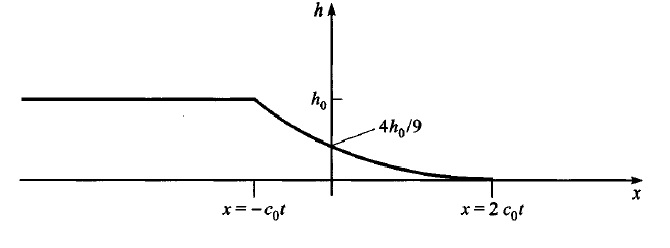
\includegraphics[scale=1]{figuras/ondalonga.jpg}	%\fbox{\includegraphics[width=.4\textwidth]{220B.jpg}}
	\caption{\textsc{O perfil da superfície livre para o tempo $t$ após a ruptura de barragens}}
	\vspace{-0.1cm}
	\legend{FONTE: \citeonline{Johnson}}
	\label{ondalonga}
\end{figure}
     



%------------------------------------------------------------------------------------------------------------------------------------------------------
\section{O CÓDIGO PySPH} \label{py}

Dentre os inúmeros códigos desenvolvidos para o método SPH destaca-se o PySPH, por ser um código aberto, com processamento em paralelo e implementado em Python, que é uma linguagem de alto nível, orientada a objeto, com programação interpretada e de fácil aprendizagem.

O PySPH foi apresentado no trabalho de \citeonline{Ramachandran2010} que desenvolveram este código com o intuito de suprir a comunidade científica com um código de fonte aberta e com repositório acessível ao público, detalhes estes que não são encontrados em outras implementações, conforme destacam os autores. 

O Python, por ser uma linguagem interpretada, torna o processamento lento. No entanto, para contornar esta dificuldade no PySPH, toda a performance crítica do processamento foi desenvolvida em Cython, que é uma linguagem escrita em C com extensões para Python, ou seja, ao compilar um módulo em Cython este é compilado em extensões C que podem ser importados para Python, agilizando todo o processo. 

De forma geral, para realizar as simulações, o PySPH utiliza poucos objetos chaves, tais como \textit{Solver}, que controla outras funções como o integrador, ou as \textit{Entities}, que são coleções de partículas que podem representar classes de entidades físicas, como fluidos ou sólidos. Uma visão simplificada deste processo pode ser visto na Figura \ref{fig:diagrama} onde estão delineadas as principais fases. Cada uma destas fases, bem como uma visão mais detalhada sobre a arquitetura do código, pode ser encontrada no repositório desenvolvidos pelos autores \citeonline{PySPH}.

\begin{figure}[H]
\centering
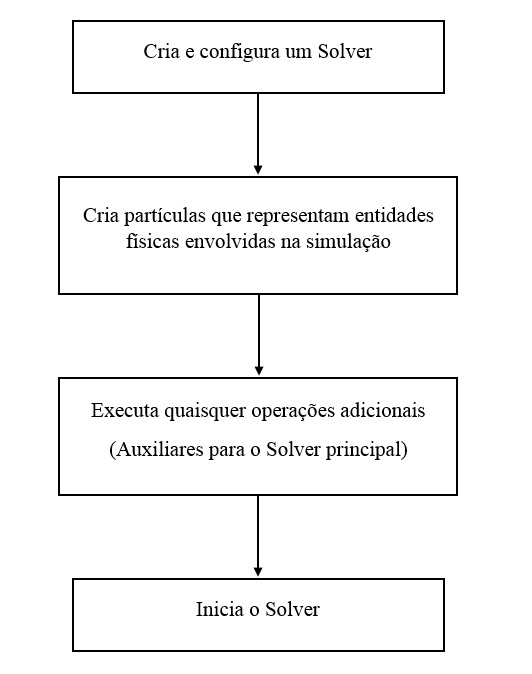
\includegraphics[scale=0.8]{figuras/diagrama.jpg}
\caption{\textsc{Esboço das tarefas executadas numa simulação em PySPH}}
\vspace{-0.1cm}
\legend{FONTE: Adaptado de \citeonline{Ramachandran2010}}
\label{fig:diagrama}
\end{figure}

A eficiência do código é comprovada por meio de alguns exemplos, entre eles está a ruptura de uma barragem hipotética seguindo o trabalho de \citeonline{Crespo}. Para tanto, consideraram a Figura \ref{fig:tanque} como representando a barragem. Como parâmetros utilizaram as condições de fronteira dinâmica e formaram um \textit{grid} de mesmo espaçamento nas direções dos eixos coordenados $x$ e $y$ de tamanho $dx=dy=0,03 \ m$. Com isso, utilizaram $4.556$ partículas representando o fluido e $671$ partículas representado as fronteiras. Utilizaram a suavização do núcleo igual a $h=0,039 \ m$ resultando em um raio de atuação do núcleo igual a $h/dx=1,3 \ m$, o que utiliza, aproximadamente, $21$ vizinhos para cada partícula por passo adotado, conforme comenta \citeonline{Liu2003}. Como tamanho de passo consideraram $dt=10^{-4}s$, com tempo total de simulação igual a $tf=1s$.

Além dos parâmetros acima destacados, \citeonline{Ramachandran2010} adotaram também a densidade da água como $\rho=1000 \ kg/m^{3}$, velocidade do som como $co=10 \times \sqrt{2 \times 9,81 \times 2} \ m/s$, $\alpha=0,5$ como fator de correção XSPH, $\gamma=7,0$ utilizada como uma constante na equação de estado e $B=co^2 \times \rho/ \gamma$ como valor para o termo relacionado às flutuações de densidade do fluido.

Das equações utilizadas em SPH para modelar a ruptura de barragens, como a equação da continuidade (\ref{Cont_SPH}) e a equação do momento (\ref{Mov_SPH}), destaca-se a equação de estado
\begin{equation} \label{estado}
P=B \left[\left(\frac{\rho}{\rho_0}\right)^{\gamma}-1\right],
\end{equation} 
que é a equação de Tait que descreve uma relação entre a pressão e a densidade \cite{Monaghan1994}. Conforme destacam \citeonline{Crespo}, a constante $\gamma$ pode variar entre $1$ e $7$, sendo que $\gamma=7$ é normalmente usada para aplicações oceânicas. Ainda, segundo esses autores, a utilização dessa equação evita o cálculo da pressão da equação de Poisson, o que reduz o esforço computacional.

Para formação dos núcleos, nesta simulação, os autores utilizaram a função Spline de quinto grau, já que este tipo de função tem um comportamento próximo de uma função gaussiana, mas não melhor que a Spline cúbica, conforme pode ser observado na Figura \ref{fig:nucleos}.

Alguns resultados para comprovar a eficiência do código PySPH, em diferentes tempos de simulação, foram obtidos para o problema modelo e serão apresentados  e discutidos na Seção \ref{REPy}. 
%obtidos podem ser observados nas figuras (\ref{fig:pysph01s}) - (\ref{fig:pysphfim}).


      

%------------------------------------------------------------------------------------------------------------------------------------------------------
\section{PROPOSTA DA PESQUISA} \label{proposta}

Como objetivo principal desta dissertação, foi proposto a modelagem computacional da ruptura de uma barragem hipotética, cujo movimento da massa líquida era governado pelas equações de Euler. Para atingir esse objetivo as equações seriam discretizadas por meio do MDFE, em associação com o esquema difusivo de Lax-Friedrichs. No entanto, conforme destaca \citeonline{Stansby}, os estágios iniciais do movimento da massa líquida são os mais importantes em toda simulação, pois são nesses instantes em que se iniciam a formação das ondas de choques ou rarefação e métodos como o MDFE, associado a esquemas difusivos, não têm um comportamento adequado para o tratamento dessas descontinuidades, já que são considerados métodos de primeira ordem \cite{Crossley}.

Para manter o objetivo do trabalho, foram obtidas as equações de Águas Rasas (\ref{ARR2}) e (\ref{AR2}) considerando o escoamento levemente compressível nas equações de Euler. Isso permitiu definir, com o auxílio do Método das Características, uma solução analítica para o perfil do escoamento nos estágios iniciais do movimento da massa líquida, equações (\ref{solzAR}) e (\ref{soluAR}).

A formulação desenvolvida nas equações (\ref{solzAR}) e (\ref{soluAR}) baseou-se na hipótese do escoamento ocorrer em canais infinitos. No entanto, essa hipótese não condiz com o modelo hipotético adotado mostrado na Figura \ref{tanque2}. Assim, as equações (\ref{solzAR}) e (\ref{soluAR}) foram adequadas para o modelo em questão, ou seja, para o caso de um canal finito. Dessa forma, considerando $h_0=2 \ m$ o perfil inicial da coluna d'água, $l=1 \ m$ a lateral esquerda do tanque e $L=4 \ m$ a lateral direita, as soluções analíticas do perfil da superfície livre $h(x,t)$ e da velocidade média do escoamento $u(x,t)$ passaram a ser determinadas por 
\begin{equation} \label{solzMod}
	h(x,t)= \frac{1}{9g} \left[2 \sqrt{gh_0} - \frac{l-x}{t} \right]^2
\end{equation}
e
\begin{equation} \label{soluMod}
	u(x,t)=2 \left[ \sqrt{gh_0} - \sqrt{gh} \right],
\end{equation}
desde que $g=9,8m/s^2$ seja a aceleração de gravidade, $l-t \sqrt{gh_0} \leq x \leq l+2t \sqrt{gh_0}$ e que $0 \leq t \leq min \left\{l/ \sqrt{gh_0}\ ,\ (L-l)/2 \sqrt{gh_0} \right\}$.

Porém, se $x<l-t \sqrt{gh_0}$, tem-se
\begin{equation} \label{solzMod1}
	h(x,t)=h_0
\end{equation}
e
\begin{equation} \label{soluMod1}
	u(x,t)=0.
\end{equation}

Para o caso em que $x>l+2t \sqrt{gh_0}$, a solução será dada por
\begin{equation} \label{solzMod2}
	h(x,t)=0
\end{equation}
e
\begin{equation} \label{soluMod2}
	u(x,t)=0.
\end{equation}

Essa solução analítica, conforme construída acima, é capaz de tratar os estágios iniciais do movimento da massa líquida, já que evita a formação de ondas de choque ou rarefação, momento crítico na simulação. Esse processo torna possível a adoção do esquema numérico proposto anteriormente, pois quando $x>l+2t \sqrt{gh_0}$ e  $t \longrightarrow \infty$ a profundidade da superfície livre atinge um valor constante, ou seja, tende a se estabilizar. Assim, a partir desse ponto, o uso do MDFE torna-se adequado e passa a utilizar, como condições iniciais, os valores de $h(x,t)$ e $u(x,t)$ obtidos analiticamente.

   
%------------------------------------------------------------------------------------------------------------------------------------------------------
\section{A GERAÇÃO DA MALHA} \label{malha}

O modelo computacional desenvolvido utilizou uma forma híbrida para resolver o problema da ruptura de barragens, já que adotou uma solução analítica, para os instantes iniciais do escoamento, juntamente com uma solução numérica para os demais momentos da simulação, o que evitou a formação das ondas de choque e/ou rarefação e tornou a solução final possível sem conduzir para resultados espúrios.

Para construção da parte analítica do modelo fez-se uso das soluções obtidas na Seção \ref{ModeloAR} com as modificações realizadas na Seção \ref{proposta}. Já para a parte numérica, o modelo utilizou, como fundamentação, as equações de Águas Rasas (\ref{ARR2}) e (\ref{AR2}), discretizadas por meio do MDFE (\ref{explícito}), resultando em
\begin{equation} \label{A}
\frac{h^{n+1}_{i}-h^{n}_{i}}{\Delta t}= - \left[h^{n}_{i} \left( \frac{u^{n}_{i+1}-u^{n}_{i-1}}{2 \Delta x} \right) + u^{n}_{i} \left( \frac{h^{n}_{i+1}-h^{n}_{i-1}}{2 \Delta h} \right) \right]
\end{equation}   
e
\begin{equation} \label{B}
\frac{u^{n+1}_{i}-u^{n}_{i}}{\Delta t}= - \left[u^{n}_{i} \left( \frac{u^{n}_{i+1}-u^{n}_{i-1}}{2 \Delta x} \right) + g \left( \frac{h^{n}_{i+1}-h^{n}_{i-1}}{2 \Delta h} \right) \right].
\end{equation}

Explicitando os termos para o tempo $t=n+1$, as equações discretas (\ref{A}) e (\ref{B}) tornaram-se iguais a
\begin{equation} \label{C}
h^{n+1}_{i} =  h^{n}_{i} - \frac{\Delta t}{2} \left[h^{n}_{i} \left( \frac{u^{n}_{i+1}-u^{n}_{i-1}}{ \Delta x} \right) + u^{n}_{i} \left( \frac{h^{n}_{i+1}-h^{n}_{i-1}}{ \Delta h} \right) \right]
\end{equation}
e
\begin{equation} \label{D}
u^{n+1}_{i} = u^{n}_{i} - \frac{\Delta t}{2} \left[u^{n}_{i} \left( \frac{u^{n}_{i+1}-u^{n}_{i-1}}{ \Delta x} \right) + g \left( \frac{h^{n}_{i+1}-h^{n}_{i-1}}{ \Delta h} \right) \right].
\end{equation}

Para simplificar o modelo, considerou-se uma discretização constante, tanto para altura da superfície livre $h$ como para direção da velocidade do escoamento $x$. Com isso, pôde-se adotar $ \Delta h = \Delta x = \Delta$ e, dessa forma, as equações (\ref{C}) e (\ref{D}) passaram a ser escritas como
\begin{equation} \label{E}
h^{n+1}_{i} =  h^{n}_{i} - \alpha \left[h^{n}_{i} \left( u^{n}_{i+1}-u^{n}_{i-1} \right) + u^{n}_{i} \left( h^{n}_{i+1}-h^{n}_{i-1} \right) \right]
\end{equation}
e
\begin{equation} \label{F}
u^{n+1}_{i} = u^{n}_{i} - \alpha \left[u^{n}_{i} \left( u^{n}_{i+1}-u^{n}_{i-1} \right) + g \left( h^{n}_{i+1}-h^{n}_{i-1} \right) \right]
\end{equation}
onde $ \alpha = { \Delta t}/{2 \Delta}$.

A aplicação do esquema difusivo de Lax-Friedrichs (\ref{ELF}) nas equações (\ref{E}) e (\ref{F}) resultou no modelo final para simulação numérica proposta, ou seja, a suavização das equações resultou em
\begin{equation} \label{G}
	\small{ h^{n+1}_{i} =0.5 \left( h^{n}_{i+1}+h^{n}_{i-1} \right)  - \alpha \left[ 0.5 \left( h^{n}_{i+1}+h^{n}_{i-1} \right) \left( u^{n}_{i+1}-u^{n}_{i-1} \right)  + 0.5 \left( u^{n}_{i+1}+u^{n}_{i-1} \right) \left( h^{n}_{i+1}-h^{n}_{i-1} \right) \right] }
\end{equation}
e
\begin{equation} \label{H}
	u^{n+1}_{i} =0.5 \left( u^{n}_{i+1}+u^{n}_{i-1} \right) - \alpha \left[ 0.5 \left( u^{n}_{i+1}+u^{n}_{i-1} \right) \left( u^{n}_{i+1}-u^{n}_{i-1} \right) + g \left( h^{n}_{i+1}-h^{n}_{i-1} \right) \right]
\end{equation}
com condições de contorno $u(0,t)=0$, $u(L,t)=0$ e condições iniciais determinadas pelas soluções analíticas da Seção \ref{ModeloAR}.

Para garantir a estabilidade do modelo, a condição (\ref{CFL}) define que
\begin{equation}
\Delta t = Co \times \Delta.
\end{equation}
Como o tanque que simula a barragem hipotética possui um comprimento de $L=4 \ m$ optou-se por considerar uma discretização total de $400$ passos na direção do escoamento, o que proporcionou um incremento infinitesimal, na direção $x$,  igual a $ \Delta = 0,01 \ m$. Assim, adotando como condição de estabilidade $Co=0,01$, obteve-se o incremento infinitesimal para o avanço no tempo igual a
\begin{equation}
\Delta t = 0,01 \times 0,01 = 0,0001s,
\end{equation}
proporcionando uma quantidade razoável de amostras para compor as médias da elevação do perfil da coluna d'água e da velocidade do escoamento, capazes de representar alguns fenômenos que surgem no problema físico. 

      







%-------------------------------------------------------------------------------------------------------------------------------------------------------

%\section{VARIAÇÃO DOS PARÂMETROS} \label{parametros}


